\documentclass[border=8pt, multi, tikz]{standalone}
\usepackage{tikz}
\usepackage{tikz-3dplot}
\usetikzlibrary{quotes,arrows.meta,positioning,3d,calc}

% Define layer colors
\def\ConvColor{rgb:yellow,5;red,2.5;white,5}
\def\ConvReluColor{rgb:yellow,5;red,5;white,5}
\def\PoolColor{rgb:red,1;black,0.3}
\def\FcColor{rgb:blue,5;red,2.5;white,5}
\def\FcReluColor{rgb:blue,5;red,5;white,4}
\def\SoftmaxColor{rgb:magenta,5;black,7}
\def\SumColor{rgb:blue,5;green,15}
\def\InputColor{rgb:gray,5;white,10}
\def\HexColor{rgb:green,5;black,3}
\def\TransColor{rgb:blue,5;white,5}

\begin{document}
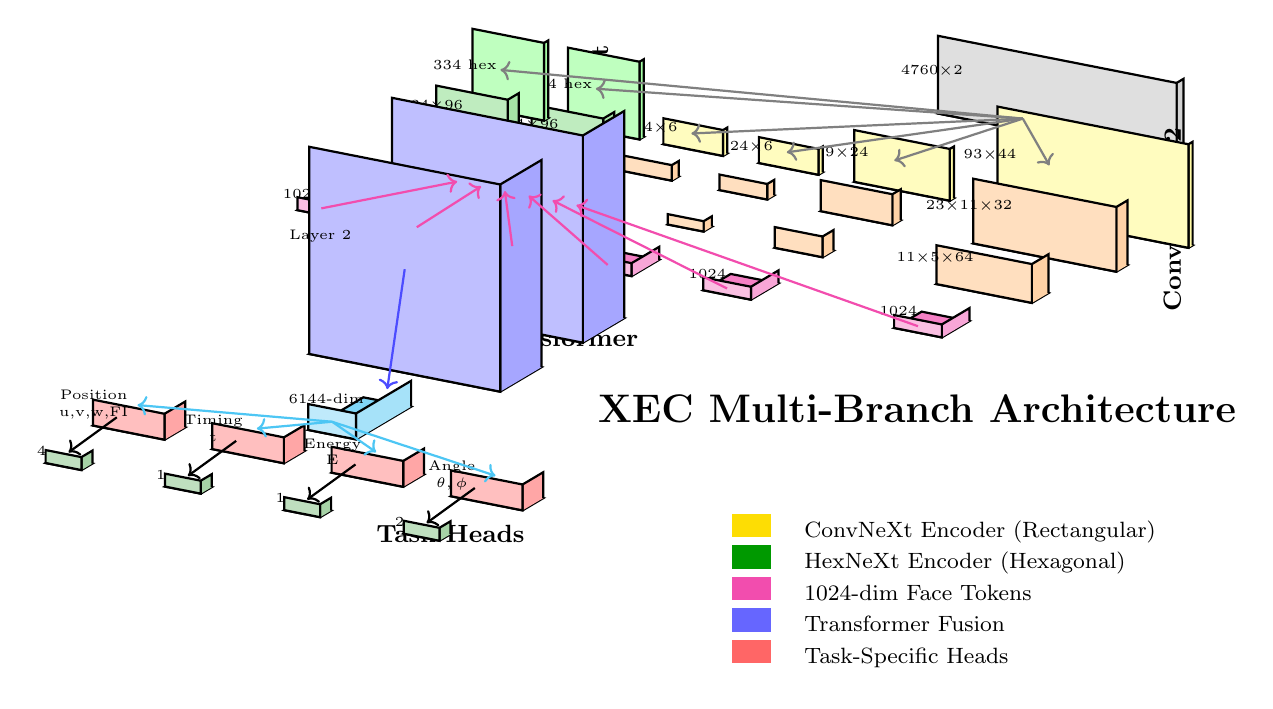
\begin{tikzpicture}
\tikzstyle{connection}=[ultra thick,every node/.style={sloped,allow upside down},draw=\edgecolor,opacity=0.7]
\tikzstyle{copyconnection}=[ultra thick,every node/.style={sloped,allow upside down},draw={rgb:blue,4;red,1;green,1;black,3},opacity=0.7]

%% Define macros for 3D boxes
% #1=name, #2=caption, #3=fill color, #4=height, #5=width, #6=depth, #7=x, #8=y
\newcommand{\Block}[8]{
    \coordinate (#1-anchor) at (#7,#8,0);
    % Front face
    \fill[#3!50] (#7,#8,0) -- (#7,#8+#4,0) -- (#7+#5,#8+#4,0) -- (#7+#5,#8,0) -- cycle;
    \draw[thick] (#7,#8,0) -- (#7,#8+#4,0) -- (#7+#5,#8+#4,0) -- (#7+#5,#8,0) -- cycle;
    % Top face
    \fill[#3!35] (#7,#8+#4,0) -- (#7,#8+#4,#6) -- (#7+#5,#8+#4,#6) -- (#7+#5,#8+#4,0) -- cycle;
    \draw[thick] (#7,#8+#4,0) -- (#7,#8+#4,#6) -- (#7+#5,#8+#4,#6) -- (#7+#5,#8+#4,0);
    % Right face
    \fill[#3!25] (#7+#5,#8,0) -- (#7+#5,#8+#4,0) -- (#7+#5,#8+#4,#6) -- (#7+#5,#8,#6) -- cycle;
    \draw[thick] (#7+#5,#8,0) -- (#7+#5,#8+#4,0) -- (#7+#5,#8+#4,#6) -- (#7+#5,#8,#6) -- cycle;
    % Label
    \node[font=\tiny, align=center] at (#7+#5/2, #8-0.4, #6/2) {#2};
}

% Set 3D view
\tdplotsetmaincoords{70}{120}
\begin{scope}[tdplot_main_coords, scale=0.35]

%% ========== TITLE ==========
\node[font=\Large\bfseries] at (25, 20, 0) {XEC Multi-Branch Architecture};

%% ========== INPUT ==========
\node[font=\small\bfseries] at (-5, 12, 0) {Input};
\Block{input}{4760$\times$2}{gray}{10}{0.5}{3}{-3}{5}

%% ========== RECTANGULAR FACE ENCODERS (ConvNeXt) ==========
\node[font=\small\bfseries, rotate=90] at (3, 18, 0) {ConvNeXt V2};

% Inner Face Path (93x44x2 -> 23x11x32 -> 11x5x64 -> 1024)
\Block{inner-in}{93$\times$44}{yellow}{8}{0.3}{4}{5}{12}
\Block{inner-s1}{23$\times$11$\times$32}{orange}{6}{0.8}{2.5}{8}{13}
\Block{inner-s2}{11$\times$5$\times$64}{orange}{4}{1.2}{1.5}{12}{14}
\Block{inner-tok}{1024}{magenta}{2}{2}{0.5}{16}{15}

% Outer Face Path (9x24x2 -> similar)
\Block{outer-in}{9$\times$24}{yellow}{4}{0.3}{2}{5}{6}
\Block{outer-s1}{}{orange}{3}{0.6}{1.2}{8}{6.5}
\Block{outer-s2}{}{orange}{2}{0.8}{0.8}{12}{7}
\Block{outer-tok}{1024}{magenta}{2}{2}{0.5}{16}{7}

% US Face Path (24x6x2)
\Block{us-in}{24$\times$6}{yellow}{2.5}{0.3}{1}{5}{2}
\Block{us-s1}{}{orange}{2}{0.5}{0.6}{8}{2.2}
\Block{us-s2}{}{orange}{1.5}{0.6}{0.4}{12}{2.4}
\Block{us-tok}{1024}{magenta}{2}{2}{0.5}{16}{2}

% DS Face Path (24x6x2)
\Block{ds-in}{24$\times$6}{yellow}{2.5}{0.3}{1}{5}{-2}
\Block{ds-s1}{}{orange}{2}{0.5}{0.6}{8}{-1.8}
\Block{ds-s2}{}{orange}{1.5}{0.6}{0.4}{12}{-1.6}
\Block{ds-tok}{1024}{magenta}{2}{2}{0.5}{16}{-2}

%% ========== HEXAGONAL FACE ENCODERS (HexNeXt) ==========
\node[font=\small\bfseries, rotate=90] at (3, -6, 0) {HexNeXt};

% Top PMT Path (334 nodes)
\Block{top-in}{334 hex}{green}{3}{0.3}{3}{5}{-6}
\Block{top-s1}{334$\times$96}{green!70!black}{3}{0.8}{2}{8}{-5.5}
\Block{top-tok}{1024}{magenta}{2}{2}{0.5}{16}{-6}

% Bottom PMT Path (334 nodes)
\Block{bot-in}{334 hex}{green}{3}{0.3}{3}{5}{-10}
\Block{bot-s1}{334$\times$96}{green!70!black}{3}{0.8}{2}{8}{-9.5}
\Block{bot-tok}{1024}{magenta}{2}{2}{0.5}{16}{-10}

%% ========== TRANSFORMER FUSION ==========
\node[font=\small\bfseries] at (25, 5, 0) {Transformer};

% Transformer blocks
\Block{trans1}{6 tokens\\8 heads}{blue}{8}{3}{8}{22}{-2}
\Block{trans2}{Layer 2}{blue}{8}{3}{8}{28}{-2}

%% ========== CONCAT ==========
\Block{concat}{6144-dim}{cyan}{2}{4}{1}{34}{2}

%% ========== TASK HEADS ==========
\node[font=\small\bfseries] at (45, 12, 0) {Task Heads};

\Block{head-ang}{Angle\\$\theta,\phi$}{red}{3}{1.5}{1}{40}{10}
\Block{head-eng}{Energy\\E}{red}{3}{1.5}{1}{40}{5}
\Block{head-tim}{Timing\\t}{red}{3}{1.5}{1}{40}{0}
\Block{head-pos}{Position\\u,v,w,FI}{red}{3}{1.5}{1}{40}{-5}

%% ========== OUTPUT ==========
\Block{out-ang}{2}{green!50!black}{1.5}{0.8}{0.5}{45}{10.5}
\Block{out-eng}{1}{green!50!black}{1.5}{0.8}{0.5}{45}{5.5}
\Block{out-tim}{1}{green!50!black}{1.5}{0.8}{0.5}{45}{0.5}
\Block{out-pos}{4}{green!50!black}{1.5}{0.8}{0.5}{45}{-4.5}

%% ========== CONNECTIONS ==========
% Input to encoders
\draw[->, thick, gray] (0,10,1.5) -- (5,14,2);
\draw[->, thick, gray] (0,10,1.5) -- (5,7.5,1);
\draw[->, thick, gray] (0,10,1.5) -- (5,3,0.5);
\draw[->, thick, gray] (0,10,1.5) -- (5,-1,0.5);
\draw[->, thick, gray] (0,10,1.5) -- (5,-5,1.5);
\draw[->, thick, gray] (0,10,1.5) -- (5,-9,1.5);

% Tokens to transformer
\draw[->, thick, magenta!70] (18,16,0.25) -- (22,4,4);
\draw[->, thick, magenta!70] (18,8,0.25) -- (22,3,4);
\draw[->, thick, magenta!70] (18,3,0.25) -- (22,2,4);
\draw[->, thick, magenta!70] (18,-1,0.25) -- (22,1,4);
\draw[->, thick, magenta!70] (18,-5,0.25) -- (22,0,4);
\draw[->, thick, magenta!70] (18,-9,0.25) -- (22,-1,4);

% Transformer to concat
\draw[->, thick, blue!70] (31,2,4) -- (34,3,0.5);

% Concat to heads
\draw[->, thick, cyan!70] (38,3,0.5) -- (40,11,0.5);
\draw[->, thick, cyan!70] (38,3,0.5) -- (40,6,0.5);
\draw[->, thick, cyan!70] (38,3,0.5) -- (40,1,0.5);
\draw[->, thick, cyan!70] (38,3,0.5) -- (40,-4,0.5);

% Heads to outputs
\draw[->, thick] (41.5,11,0.5) -- (45,11,0.25);
\draw[->, thick] (41.5,6,0.5) -- (45,6,0.25);
\draw[->, thick] (41.5,1,0.5) -- (45,1,0.25);
\draw[->, thick] (41.5,-4,0.5) -- (45,-4,0.25);

\end{scope}

%% ========== LEGEND ==========
\node[font=\footnotesize, anchor=north west] at (-1, -5) {
    \begin{tabular}{ll}
    \textcolor{yellow!80!orange}{\rule{0.5cm}{0.3cm}} & ConvNeXt Encoder (Rectangular) \\
    \textcolor{green!60!black}{\rule{0.5cm}{0.3cm}} & HexNeXt Encoder (Hexagonal) \\
    \textcolor{magenta!70}{\rule{0.5cm}{0.3cm}} & 1024-dim Face Tokens \\
    \textcolor{blue!60}{\rule{0.5cm}{0.3cm}} & Transformer Fusion \\
    \textcolor{red!60}{\rule{0.5cm}{0.3cm}} & Task-Specific Heads \\
    \end{tabular}
};

\end{tikzpicture}
\end{document}
